% Discription of what ROS is and what it does

\chapter{Robot Operating System\authorA} \label{ref:ros}

\section{What is the Robot Operating System?}
The Robot Operating System\footnote{ROS and/or the "nine dots" ROS logo and/or any other ROS trademarks are a trademark of Open Robotics}, which is also known as \gls{ros}\texttrademark  is a flexible framework for writing software that gets utilized on robots. It was founded by Willow Garage in 2012 and gets primarily maintained by the \href{https://www.openrobotics.org/}{Open Source Robot Foundation} (\gls{osrf}) \cite{osrf}. In Europe the project gets coordinated by the Fraunhofer IPA in form of the \href{https://rosindustrial.org/ric-eu}{\gls{ros} Industrial Consortium Europe} \cite{rosice}. \gls{ros} is a middle-ware which is not an operating system but provides services that handles passing messages between processes, package management and hardware abstraction. \emph{\enquote{It is a collection of tools, libraries, and conventions that aim to simplify the task of creating complex and robust robot behavior across a wide variety of robotic platforms.}} \cite{aboutros} \newline
\begin{figure}[h]
	\centering
	
\includegraphics[width=0.5\textwidth]{./media/images/ros_logo.eps}
  	\caption{"Nine dots"\texttrademark  \gls{ros} logo}
  	\label{rosstructure}
\end{figure}

\section{Design}
The processes of \gls{ros} are represented in nodes which are in a graph structure. Everything gets managed by a single process called \textit{\gls{ros} Master}, to whom all other nodes register on startup, tell what they publish or on which topic they want to subscribe on. But instead of sending all of the messages over the master, the master sets up a peer-to-peer connection between the nodes which then looks like figure \ref{rosstructure}. Services are a bit different since a node directly connects to another node using the service instead of a publicly available topic. This decentralized architecture is helpful as many robots consists of many computer hardware which is connected via a network and are likely to transfer big messages \cite{rosoneoone}.\newline
For example the publisher and subscriber nodes in figure \ref{rosstructure} first register at the \gls{ros} master. Afterwards the publisher node publishes data like a image on a specific topic like \textit{image}. When a node wants to subscribe to a certain topic the \gls{ros} master first checks if another node is publishing on the topic. If that is not the case the \gls{ros} master will return an error. If the topic gets published the master creates a connection between the publisher and the subscriber. The messages that are able to contain pretty much every datatype are set over such a connection until. It is important to keep in mind that the publisher node only starts sending messages when another node actually subscribes an thus saves bandwidth when a publisher node has no subscribers.\newline
\begin{figure}[h]
	\centering
	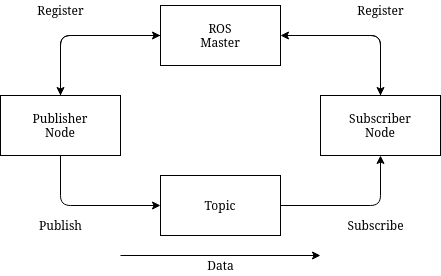
\includegraphics[height=0.5\textwidth]{./media/images/rosstructure.png}
  	\caption{\gls{ros} structure}
  	\label{rosstructure}
\end{figure}

\subsection{Topics}
It is based on a topic system, where a topic acts like a bus over which nodes send and receive messages. Each topic must be unique in its name, which is usually set by the developer. The process of publishing and subscribing is handles anonymously so that no node knows which nodes are sending and receiving messages on a certain topic. When a node wants to subscribe onto a specific topic it communicates with the \textit{\gls{ros} master}. If another node publishes on this topic the master connects the two nodes with each other in a peer-to-peer design.

\subsection{Nodes}
A node, which represents a single running process, can provide data using a matching topic and publishes it to the system, where theoretically every other node can subscribe to it, to get the data. 

\subsection{Services} \label{ref:rosservice}
Nodes can also advertise services which contain a single action. For example a node that publishes a video might contain a service which only returns the first, current or last frame. They are used for commands that are not used frequently or don't process much data.

\subsection{Parameter server}
A parameter server is like a database where all nodes have static or semi-static access to information. The data can be settings or fixed variables like distance or weight.

\section{Licenses and OS}
The language-independent tools and the main client libraries have been released under the BSD license and as such they are open source software for commercial and research use. The majority of 3rd party packages are released under several other open-source licenses.\newline
The \gls{ros} libraries are geared toward a UNIX-System which is mainly due to their dependence on a large collection of open source software and libraries.
For example \textit{Ubuntu} is in the list of supported operating systems, while others like \textit{Fedora, Mac OS and Windows} are \enquote{experimental} and are mainly supported by the community \cite{isrosforme}.

\section{Tools}
One of the core functionalities that \gls{ros} provides are the tools which allow the developers to visualize 2D and 3D data, record data, easily navigating \gls{ros} packages, creating complex scripts that configure and setup processes. This tool simplifies the workflow and provides solution for common robotic development.

\subsection{Rosbag}
Rosbag is a tool that can be used via the command line to record, playback and store \gls{ros} message data. When starting a recording all the published data gets stored in a so called bag-file. This makes it possible to record all published topics and then artificially run them later again. By doing this the recorded messages get published into the system, as if they were live. It's very handy if you need data for later development or to test nodes on different scenarios that come across later.

\subsection{RQt}\label{rqt}
RQt provides a graphical overview of the \gls{ros} computation graph. It shows the nodes and how they are connected to each other. It also shows if a node is even subscribing to a topic or publishes something. Other than that it can be used to subscribe to different topics and show them directly in RQt.\newline
\begin{figure}[h]
	\centering
	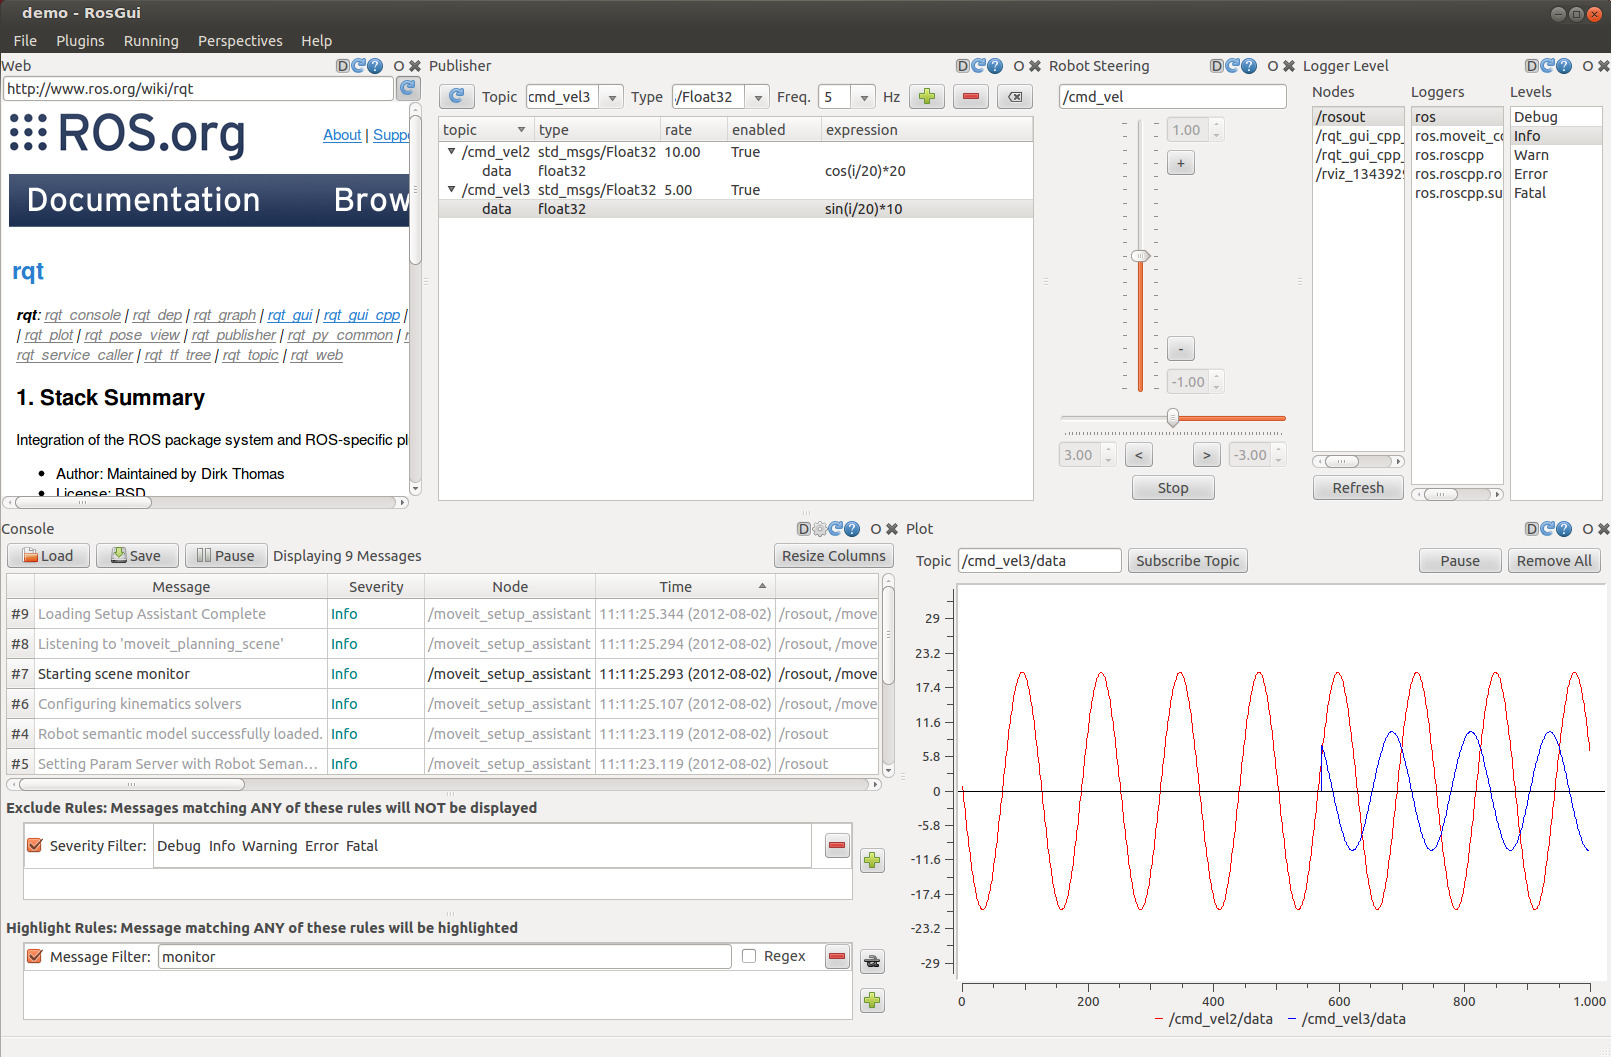
\includegraphics[width=0.7\textwidth]{./media/images/RQt}
  	\caption{RQt interface\\Src: \url{https://wiki.ros.org/RQt}}
  	\label{rqtinterface}
\end{figure}

\subsection{CatKin}\label{catkin}
Catkin is the newer \gls{ros} build system, which compiles the files in the source folder. It is based on CMake and is cross-platform and language-independent as most other \gls{ros} tools.

\subsection{Rviz}\label{rviz}
A visualizer for three-dimensional position-data where robots, environments and sensor information can be visualized. It is highly customizable and is able to display many different types of incoming data. The typical interface on startup looks similar to figure \ref{rvizinterface}. On the left are the subscribed topics and on the right are settings for displaying the incoming information. \newline
\begin{figure}[h]
	\centering
	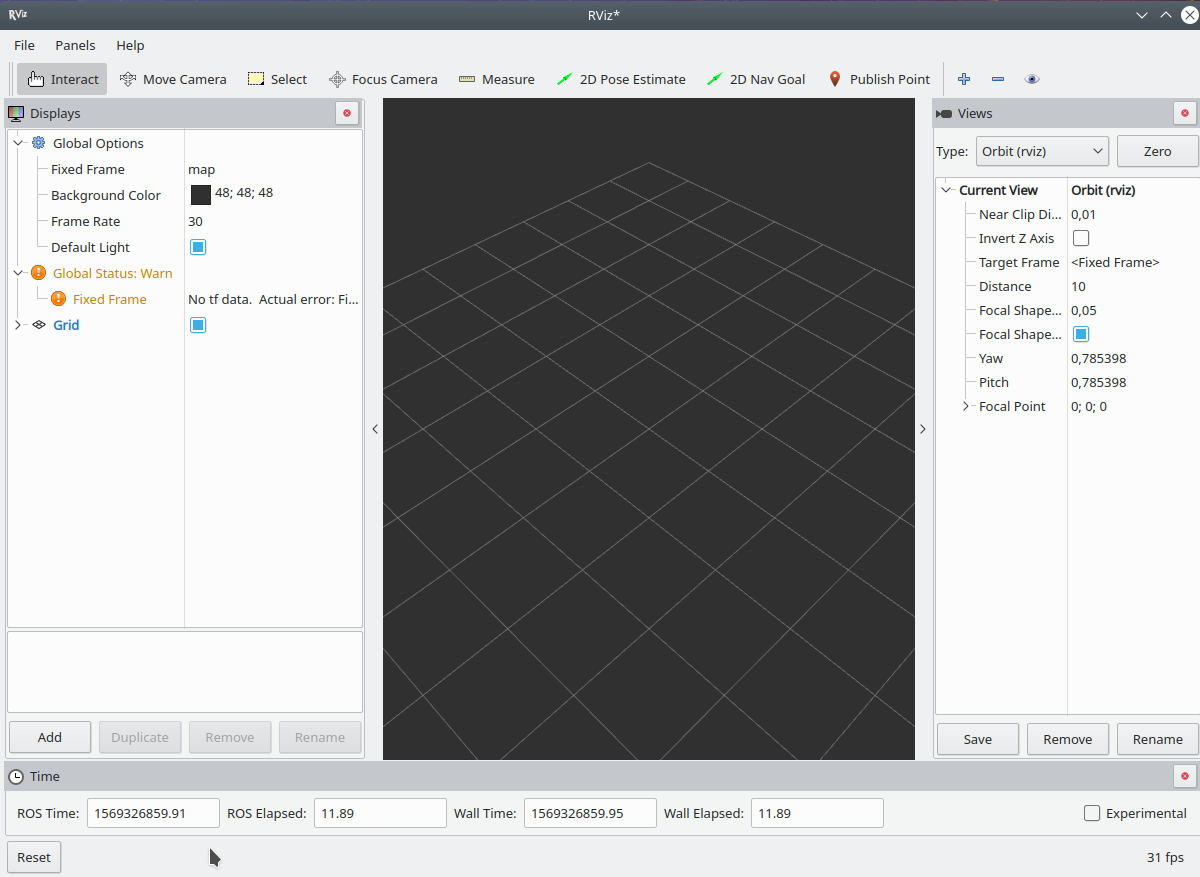
\includegraphics[width=0.7\textwidth]{./media/images/rviz}
  	\caption{Rviz interface}
  	\label{rvizinterface}
\end{figure}

\subsection{Roslaunch}\label{roslaunch}
Roslaunch is a tool for launching multiple \gls{ros} nodes and setting parameters on startup. It can be used to launch nodes locally or remotely on a server.
The configuration for a start script is written in a launch file using XML. In these files it is easy to make a automated startup and configuration process to be executed with one command. It is also possible to execute launch files in other launch files to chain them together and therefore start a complete system in the correct order with a single launch file.